\documentclass[a4paper, 10pt, final, garamond]{book}
\usepackage{cours-preambule}

\makeatletter
\renewcommand{\@chapapp}{Devoir surveill\'e -- num\'ero}
\makeatother

\begin{document}
\setcounter{chapter}{6}

\chapter{Commentaires sur le DS n\degree07}
\section{Commentaires généraux}

Ce DS avait une partie très proche du cours qui a globalement été bien traitée,
mais c'est dommage que ça ne soit que pour une partie de la classe. Certaimes se
sont pris un mur…
\smallbreak
Mis à part deux ou trois copies, vous avez complètement abandonné la pratique
d'écrire les applications numériques en détaillant les valeurs. J'incluerai un
\textbf{bonus systématique} pour le prochain DS, c'est important de bien le
faire. Notamment, beaucoup de réponses ne se souciaient plus du tout du nombre
de chiffres significatifs. J'ai mis des malus pour les abus (5 au lieu de 3),
mais pas pour les petits écarts~; il y aura beaucoup plus de \textbf{malus
systématiques} pour le prochain DS.
\smallbreak
Dans l'ensemble correct mais trop peu de tentatives réussies en-dehors du cours.
10 de moyenne.

\begin{figure}[htbp!]
	\centering
	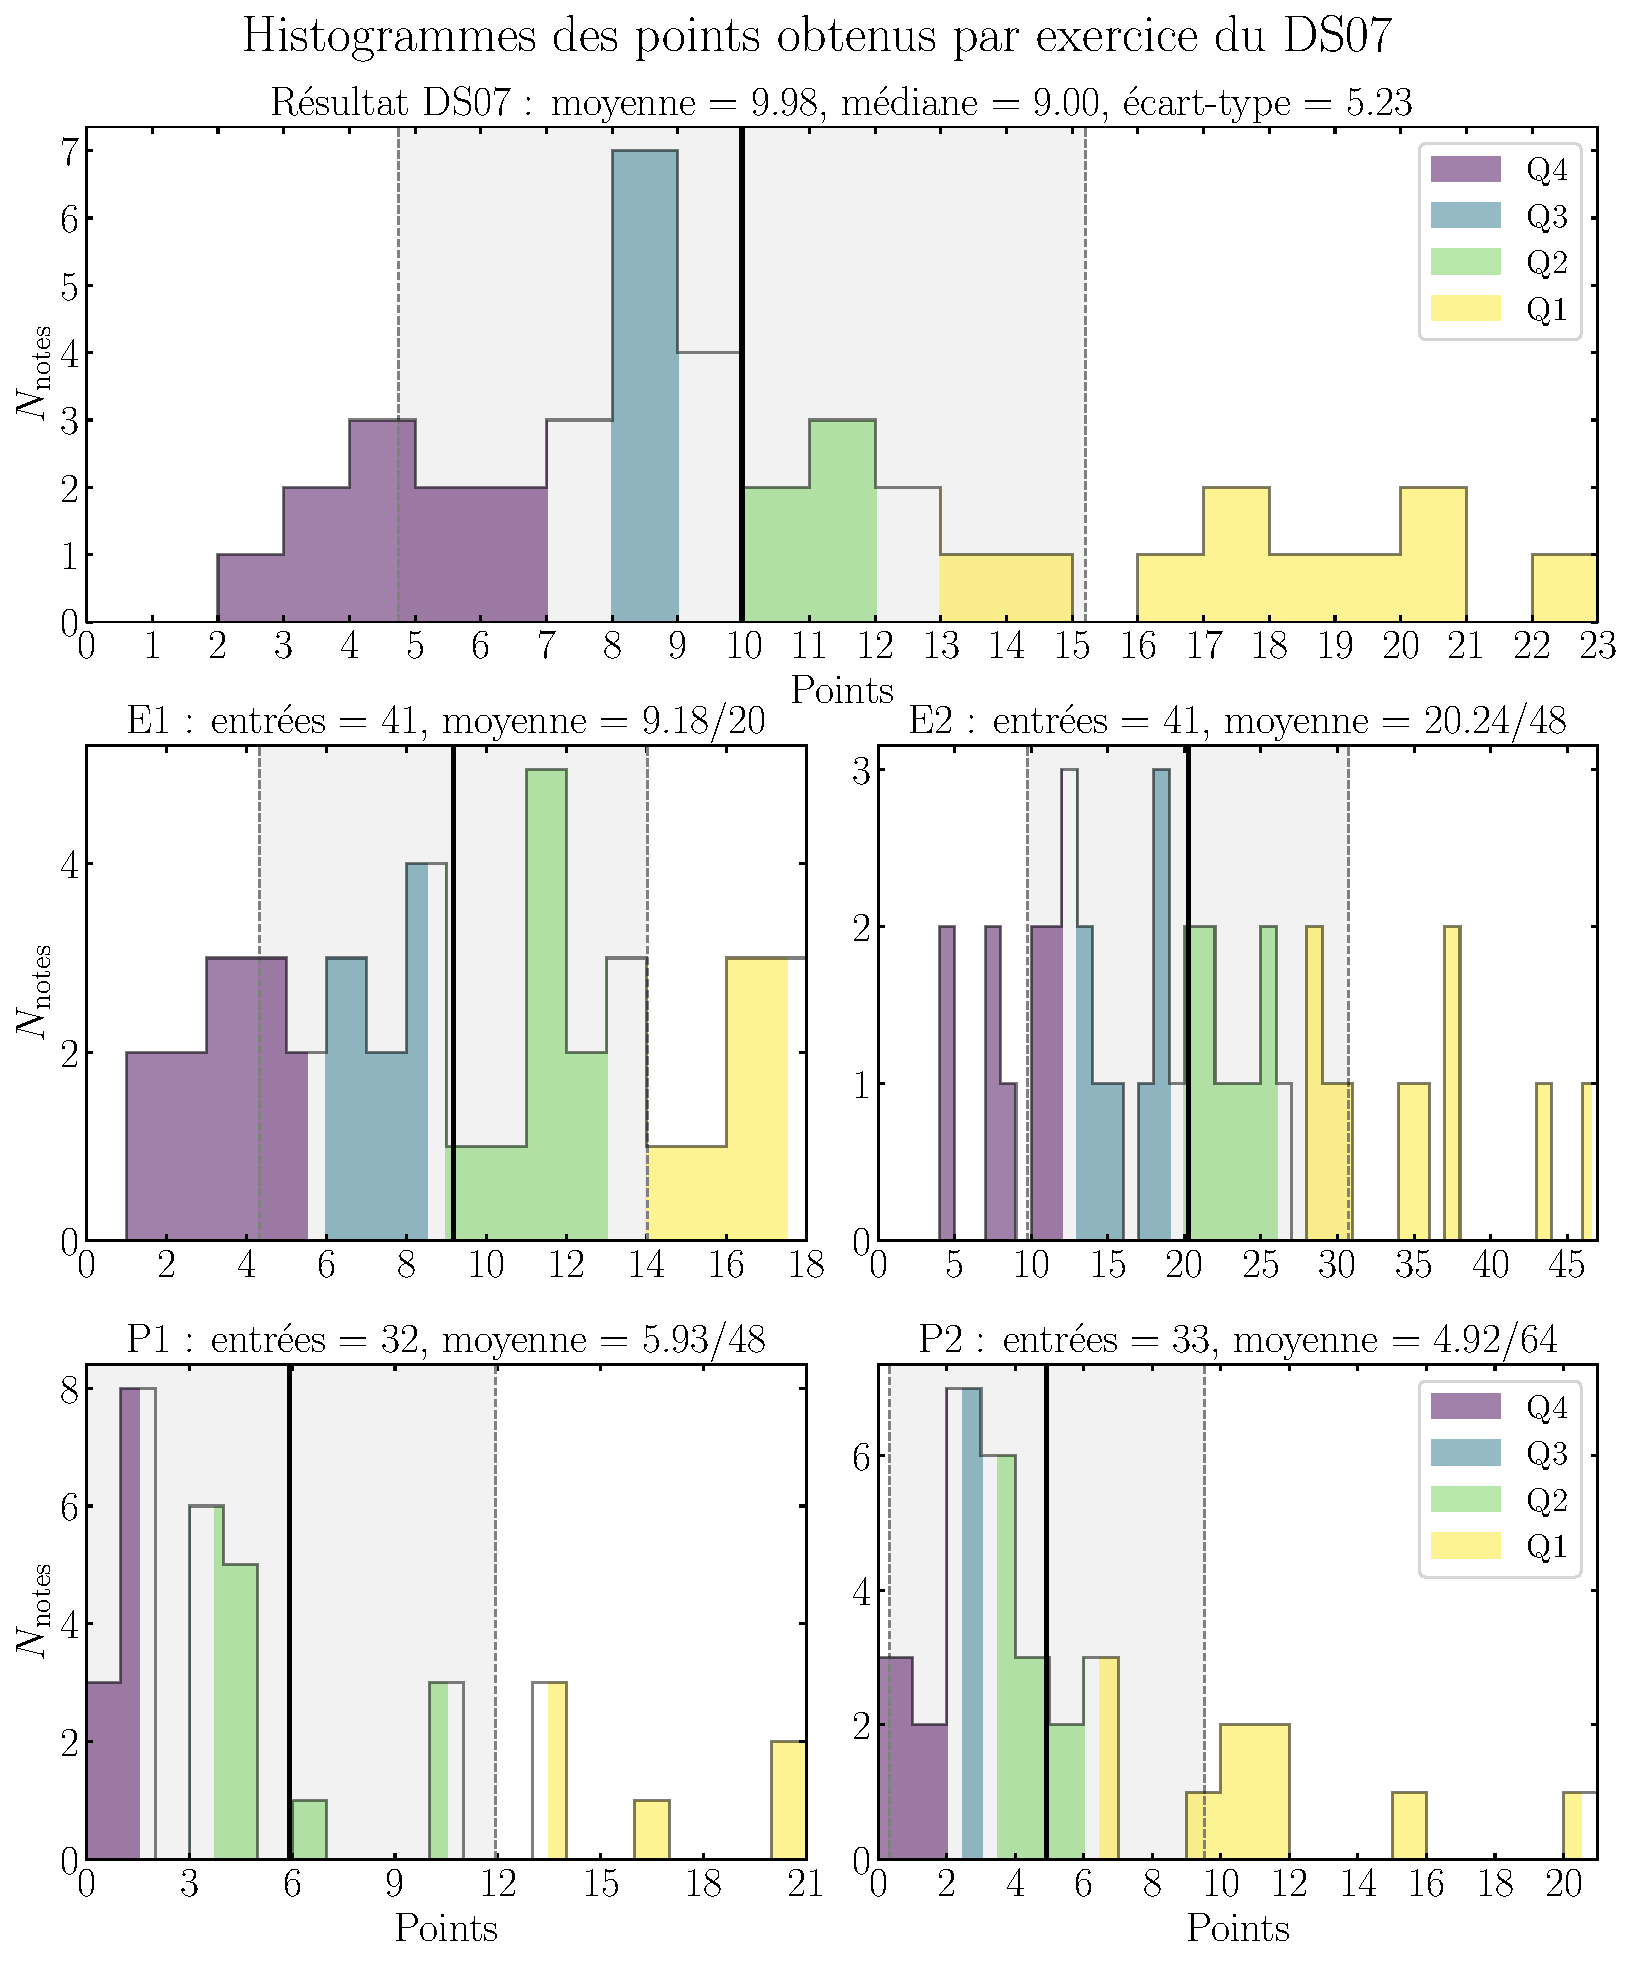
\includegraphics[width=.8\linewidth]{DS07_hist_all}
\end{figure}

\setcounter{section}{0}
\exercice[20]{Oscillations d'un métronome}
L'établissement du système était primordial ici. Cet exercice est particulier en
ce qu'on traite un solide (puisqu'on donne son moment d'inertie), mais avec une
approche des forces par la mécanique du point. Ceci étant dit, il est trait
pour trait similaire au premier exercice du TDM6 avec Archimède. Soyez conscientz
de ce que vos équations signifient et renforcez vos capacités d'analyse.
\begin{enumerate}
	\nitem{2}% Q1
	Dans l'idée correcte, mais des formulations hasardeuses. Beaucoup d'inversions
	alors que, pour rappel, $J$ est l'analogue de $m$ la masse~; donc plus $J$
	augmente plus il est compliqué de faire varier la vitesse du système.
	\nitem{8}% Q2
	Attention à la définition du système, et donc du point d'application ! Si vous
	définissez un poids $\Pf_1 = m\gf$, c'est qu'il s'applique sur le corps de
	masse $m$, pas à un barycentre imaginaire…
	\smallbreak
	De très bons schémas~: forces, bras de levier, moments représentés. Beaucoup
	incomplets.
	\smallbreak
	Attention à ne pas dire que $d$ du bras de levier vaut $- \ell\sin(\th)$~:
	\textbf{une distance est toujours positive}~! Le signe du moment scalaire
	vient de la projection du moment vecteur sur l'axe de rotation.
	\smallbreak
	Par ailleurs, l'expression $\pm d \norm{\Ff}$ ne vaut \textbf{que pour le
		moment scalaire}~!
	\bigbreak
	$\Gf$ n'est \textbf{pas une force}, c'est un couple donc un \textbf{moment}.
	\smallbreak
	Pas de tension dans un solide (forces intérieures).
	\item[] RAS sur le reste.
\end{enumerate}

\exercice[47]{Satellite en orbite terrestre}
Des résultats sortis par cœur mais sans analyse de leur signification.
\begin{enumerate}
	\nitem{5}% Q1
	Définitions non connues.
	\nitem{4}% Q2
	Bien, mais il faut définir $\ur$. Énormément de personnes ont oublié le
	$1/r^{\boxed{2}}$~!! Et beaucoup trop ont répondu que la Terre ne subissait
	pas de force de la part du satellite. RIP \textsc{Newton}.
	\nitem{7}% Q3
	\textbf{Ne confondez pas moment cinétique et moment d'une force}~: $\Lcf(\Ff)$
	n'a aucun sens. Pour rappel, $\Lcf(\Sc)$ est la quantité de rotation du
	\textbf{système}, telle que $\Lcf(\Sc) = \OM \wedge \pf$ avec $\pf =
		m\vf(\Mr)$ la quantité de mouvement. Il ne vous viendrait pas à l'esprit de
	parler de la quantité de mouvement d'une force… c'est pareil pour la quantité
	de rotation. Le moment d'une force c'est $\Mcf(\Ff)$.
	\smallbreak
	Question trait pour trait égale à la question d'interrogation répétée avant et
	après les vacances. Décevant qu'elle soit souvent esquivée ou mal traitée,
	mais il y a eu quelques démonstrations par la loi des aires intéressantes
	(même si aucune n'est tout à fait convaincante).
	\nitem{4}% Q4
	Ne supposez pas que la vitesse est constante sans le montrer (par exemple avec
	\textsc{Frenet} sans $\dv{v}{t}$).
	\nitem{2}% Q5
	RAS.
	\nitem{3}% Q6
	On étudie la rotation d'un satellite \textbf{autour} de la Terre, pas de la
	Terre autour du Soleil, donc $T \neq \SI{365}{jours}$~! J'ai compté le point
	pour celleux qui ont recopié « par pure connaissance » la donnée du problème
	2, mais la seule démonstration utilisant les connaissances sur les satellites
	géostationnaires est parfaite. Personne ne connaît la distance Terre-Lune~?
	\nitem{3}% Q7
	RAS.
	\nitem{4}% Q8
	Bravo, vous avez bien intégré le lien entre force conservative et énergie
	potentielle~!
	\smallbreak
	Bien que le produit d'une force centrale avec $\dd{\OM}$ ne donne que la
	composante sur $\ur$, le déplacement élémentaire \textbf{n'est pas
		$\dd{r}\ur$}~!
	\smallbreak
	Intégrez \textbf{avec la constante} puis justifiez sa nullité.
	\nitem{10}% Q9
	Manque souvent de détails. Lisez les questions en entier. Attention au calcul
	de $v^2$~: j'ai vu d'innombrables $v^2 = (\rp + r\rp)^2$~! Soit avec des
	bonnes réponses ensuite, soit pas, mais il faut savoir calculer une norme
	corretement.
	\smallbreak
	Globalement, si vous avez passé cette question il faut reprendre le chapitre
	M7, c'est le cœur de ce chapitre.
	\nitem{5}% Q10
	RAS.
\end{enumerate}

\setcounter{section}{0}
\prblm[48]{Rotation d'un œuf dur}
\begin{enumerate}
	\nitem{2}% Q1
	Mauvaises interprétations, ou explications trop verbeuses.
	\nitem{2}% Q2
	Depuis que je vous ai dit de faire attention au signe de l'énergie
	potentielle, vous pensez qu'il y a toujours un signe $«~-~»$… l'énergie
	potentielle \textbf{augmente avec l'altitude}, peu importe le système de
	coordonnées~!
	\nitem{3}% Q3
	Erreur de calcul courante avec le $\frac{1}{5} - \frac{1}{10}$. De plus, il
	faut voir la simplification des identités remarquables $(b-a)/(b^2-a^2)$.
	\nitem{2}% Q4
	RAS
	\nitem{3}% Q5
	\textbf{Au premier ordre} est le vocabulaire que vous connaissez des
	mathématiques. Préparez-vous à faire pléthore de DL en physique… jusqu'en
	physique des particules.
	\nitem{7}% Q6
	Quelques analyses physiques intéressantes, le problème est globalement
	compris et bien mentalement représenté.
	\nitem{4}% Q7
	Idem.
	\nitem{5}% Q8
	Aucun calcul mais idem sur le signe du couple.
	\nitem{4}% Q9
	RAS.
\end{enumerate}

\prblm[64]{Satellites de télécommunication}
Vous ne pouvez pas utiliser des exercices indépendants pour obtenir les points
de questions similaires~!
\begin{enumerate}
	\nitem{9}% Q1
	Établir = \xul{démontrer}. $h$ est l'altitude, donc \textbf{pas} la distance
	entre le centre de la Terre et le satellite.
	\nitem{2}% Q2
	Ne confondez pas l'énergie potentielle de pesanteur et l'énergie potentielle
	gravitationnelle~!
	\nitem{5}% Q3
	Une unique vraie bonne réponse.
	\nitem{3}% Q4
	Exercice très intéressant à partir de cette question, mais très peu traitée.
	Une seule bonne réponse au niveau numérique (2 avec la meilleure explication
	du nombre en prenant l'arrondi supérieur).
	\nitem{3}% Q5
	Question non comprise. Faites des schémas~!
	\nitem{7}% Q6
	RAS.
	\nitem{5}% Q7
	Ne confondez pas unité ($[\ell] = \si{m}$) et dimension ($\dim{\ell} = L$).
	Questions on ne peut plus intéressantes à partir de celle-ci, ce sujet est
	très beau je vous le conseille.
	\nitem{8}% Q8
	Non traitée. Le corrigé pourra vous enrichir.
	\nitem{7}% Q9
	Non traitée.
	\nitem{2}% Q10
	Quelques tentatives mais il faut savoir calculer une norme…
	\nitem{5}% Q11
	Non traitée.
	\nitem{8}% Q12
	2 bonnes idées sur l'ensemble des copies, 1 qui a avancé dans les calculs.
\end{enumerate}

\end{document}
